% Options for packages loaded elsewhere
% Options for packages loaded elsewhere
\PassOptionsToPackage{unicode}{hyperref}
\PassOptionsToPackage{hyphens}{url}
%
\documentclass[
  ignorenonframetext,
]{beamer}
\newif\ifbibliography
\usepackage{pgfpages}
\setbeamertemplate{caption}[numbered]
\setbeamertemplate{caption label separator}{: }
\setbeamercolor{caption name}{fg=normal text.fg}
\beamertemplatenavigationsymbolsempty
% remove section numbering
\setbeamertemplate{part page}{
  \centering
  \begin{beamercolorbox}[sep=16pt,center]{part title}
    \usebeamerfont{part title}\insertpart\par
  \end{beamercolorbox}
}
\setbeamertemplate{section page}{
  \centering
  \begin{beamercolorbox}[sep=12pt,center]{section title}
    \usebeamerfont{section title}\insertsection\par
  \end{beamercolorbox}
}
\setbeamertemplate{subsection page}{
  \centering
  \begin{beamercolorbox}[sep=8pt,center]{subsection title}
    \usebeamerfont{subsection title}\insertsubsection\par
  \end{beamercolorbox}
}
% Prevent slide breaks in the middle of a paragraph
\widowpenalties 1 10000
\raggedbottom
\AtBeginPart{
  \frame{\partpage}
}
\AtBeginSection{
  \ifbibliography
  \else
    \frame{\sectionpage}
  \fi
}
\AtBeginSubsection{
  \frame{\subsectionpage}
}
\usepackage{iftex}
\ifPDFTeX
  \usepackage[T1]{fontenc}
  \usepackage[utf8]{inputenc}
  \usepackage{textcomp} % provide euro and other symbols
\else % if luatex or xetex
  \usepackage{unicode-math} % this also loads fontspec
  \defaultfontfeatures{Scale=MatchLowercase}
  \defaultfontfeatures[\rmfamily]{Ligatures=TeX,Scale=1}
\fi
\usepackage{lmodern}

\ifPDFTeX\else
  % xetex/luatex font selection
\fi
% Use upquote if available, for straight quotes in verbatim environments
\IfFileExists{upquote.sty}{\usepackage{upquote}}{}
\IfFileExists{microtype.sty}{% use microtype if available
  \usepackage[]{microtype}
  \UseMicrotypeSet[protrusion]{basicmath} % disable protrusion for tt fonts
}{}
\makeatletter
\@ifundefined{KOMAClassName}{% if non-KOMA class
  \IfFileExists{parskip.sty}{%
    \usepackage{parskip}
  }{% else
    \setlength{\parindent}{0pt}
    \setlength{\parskip}{6pt plus 2pt minus 1pt}}
}{% if KOMA class
  \KOMAoptions{parskip=half}}
\makeatother

\usepackage{color}
\usepackage{fancyvrb}
\newcommand{\VerbBar}{|}
\newcommand{\VERB}{\Verb[commandchars=\\\{\}]}
\DefineVerbatimEnvironment{Highlighting}{Verbatim}{commandchars=\\\{\}}
% Add ',fontsize=\small' for more characters per line
\usepackage{framed}
\definecolor{shadecolor}{RGB}{241,243,245}
\newenvironment{Shaded}{\begin{snugshade}}{\end{snugshade}}
\newcommand{\AlertTok}[1]{\textcolor[rgb]{0.68,0.00,0.00}{#1}}
\newcommand{\AnnotationTok}[1]{\textcolor[rgb]{0.37,0.37,0.37}{#1}}
\newcommand{\AttributeTok}[1]{\textcolor[rgb]{0.40,0.45,0.13}{#1}}
\newcommand{\BaseNTok}[1]{\textcolor[rgb]{0.68,0.00,0.00}{#1}}
\newcommand{\BuiltInTok}[1]{\textcolor[rgb]{0.00,0.23,0.31}{#1}}
\newcommand{\CharTok}[1]{\textcolor[rgb]{0.13,0.47,0.30}{#1}}
\newcommand{\CommentTok}[1]{\textcolor[rgb]{0.37,0.37,0.37}{#1}}
\newcommand{\CommentVarTok}[1]{\textcolor[rgb]{0.37,0.37,0.37}{\textit{#1}}}
\newcommand{\ConstantTok}[1]{\textcolor[rgb]{0.56,0.35,0.01}{#1}}
\newcommand{\ControlFlowTok}[1]{\textcolor[rgb]{0.00,0.23,0.31}{\textbf{#1}}}
\newcommand{\DataTypeTok}[1]{\textcolor[rgb]{0.68,0.00,0.00}{#1}}
\newcommand{\DecValTok}[1]{\textcolor[rgb]{0.68,0.00,0.00}{#1}}
\newcommand{\DocumentationTok}[1]{\textcolor[rgb]{0.37,0.37,0.37}{\textit{#1}}}
\newcommand{\ErrorTok}[1]{\textcolor[rgb]{0.68,0.00,0.00}{#1}}
\newcommand{\ExtensionTok}[1]{\textcolor[rgb]{0.00,0.23,0.31}{#1}}
\newcommand{\FloatTok}[1]{\textcolor[rgb]{0.68,0.00,0.00}{#1}}
\newcommand{\FunctionTok}[1]{\textcolor[rgb]{0.28,0.35,0.67}{#1}}
\newcommand{\ImportTok}[1]{\textcolor[rgb]{0.00,0.46,0.62}{#1}}
\newcommand{\InformationTok}[1]{\textcolor[rgb]{0.37,0.37,0.37}{#1}}
\newcommand{\KeywordTok}[1]{\textcolor[rgb]{0.00,0.23,0.31}{\textbf{#1}}}
\newcommand{\NormalTok}[1]{\textcolor[rgb]{0.00,0.23,0.31}{#1}}
\newcommand{\OperatorTok}[1]{\textcolor[rgb]{0.37,0.37,0.37}{#1}}
\newcommand{\OtherTok}[1]{\textcolor[rgb]{0.00,0.23,0.31}{#1}}
\newcommand{\PreprocessorTok}[1]{\textcolor[rgb]{0.68,0.00,0.00}{#1}}
\newcommand{\RegionMarkerTok}[1]{\textcolor[rgb]{0.00,0.23,0.31}{#1}}
\newcommand{\SpecialCharTok}[1]{\textcolor[rgb]{0.37,0.37,0.37}{#1}}
\newcommand{\SpecialStringTok}[1]{\textcolor[rgb]{0.13,0.47,0.30}{#1}}
\newcommand{\StringTok}[1]{\textcolor[rgb]{0.13,0.47,0.30}{#1}}
\newcommand{\VariableTok}[1]{\textcolor[rgb]{0.07,0.07,0.07}{#1}}
\newcommand{\VerbatimStringTok}[1]{\textcolor[rgb]{0.13,0.47,0.30}{#1}}
\newcommand{\WarningTok}[1]{\textcolor[rgb]{0.37,0.37,0.37}{\textit{#1}}}

\usepackage{longtable,booktabs,array}
\newcounter{none} % for unnumbered tables
\usepackage{calc} % for calculating minipage widths
\usepackage{caption}
% Make caption package work with longtable
\makeatletter
\def\fnum@table{\tablename~\thetable}
\makeatother
\usepackage{graphicx}
\makeatletter
\newsavebox\pandoc@box
\newcommand*\pandocbounded[1]{% scales image to fit in text height/width
  \sbox\pandoc@box{#1}%
  \Gscale@div\@tempa{\textheight}{\dimexpr\ht\pandoc@box+\dp\pandoc@box\relax}%
  \Gscale@div\@tempb{\linewidth}{\wd\pandoc@box}%
  \ifdim\@tempb\p@<\@tempa\p@\let\@tempa\@tempb\fi% select the smaller of both
  \ifdim\@tempa\p@<\p@\scalebox{\@tempa}{\usebox\pandoc@box}%
  \else\usebox{\pandoc@box}%
  \fi%
}
% Set default figure placement to htbp
\def\fps@figure{htbp}
\makeatother





\setlength{\emergencystretch}{3em} % prevent overfull lines

\providecommand{\tightlist}{%
  \setlength{\itemsep}{0pt}\setlength{\parskip}{0pt}}



 


\makeatletter
\@ifpackageloaded{caption}{}{\usepackage{caption}}
\AtBeginDocument{%
\ifdefined\contentsname
  \renewcommand*\contentsname{Table of contents}
\else
  \newcommand\contentsname{Table of contents}
\fi
\ifdefined\listfigurename
  \renewcommand*\listfigurename{List of Figures}
\else
  \newcommand\listfigurename{List of Figures}
\fi
\ifdefined\listtablename
  \renewcommand*\listtablename{List of Tables}
\else
  \newcommand\listtablename{List of Tables}
\fi
\ifdefined\figurename
  \renewcommand*\figurename{Figure}
\else
  \newcommand\figurename{Figure}
\fi
\ifdefined\tablename
  \renewcommand*\tablename{Table}
\else
  \newcommand\tablename{Table}
\fi
}
\@ifpackageloaded{float}{}{\usepackage{float}}
\floatstyle{ruled}
\@ifundefined{c@chapter}{\newfloat{codelisting}{h}{lop}}{\newfloat{codelisting}{h}{lop}[chapter]}
\floatname{codelisting}{Listing}
\newcommand*\listoflistings{\listof{codelisting}{List of Listings}}
\makeatother
\makeatletter
\makeatother
\makeatletter
\@ifpackageloaded{caption}{}{\usepackage{caption}}
\@ifpackageloaded{subcaption}{}{\usepackage{subcaption}}
\makeatother

\usepackage{bookmark}
\IfFileExists{xurl.sty}{\usepackage{xurl}}{} % add URL line breaks if available
\urlstyle{same}
% fallback for those not using the hyperref driver hyperxmp:
\makeatletter
\@ifundefined{xmpquote}{\newcommand{\xmpquote}[1]{#1}}{}
\makeatother
\hypersetup{
  pdftitle={Rejection Sampling},
  hidelinks,
  pdfcreator={LaTeX via pandoc}}


\title{\texorpdfstring{Rejection Sampling}{Rejection Sampling}}
\subtitle{\texorpdfstring{Gaussian Envelope vs.~Piecewise
Log-Affine}{Gaussian Envelope vs.~Piecewise Log-Affine}}
\author{}
\date{}

\begin{document}
\frame{\titlepage}


\begin{frame}{Overview}
\protect\phantomsection\label{overview}
\begin{itemize}
\item
  The target distribution
\item
  Method 1: Gaussian envelope
\item
  Method 2: Piecewise log-affine envelope
\item
  Comparison
\end{itemize}
\end{frame}

\begin{frame}{The Target Distribution}
\protect\phantomsection\label{the-target-distribution}
We want to sample from

\[
f(y) \propto q(y) = \exp\left(\sum_{i=1}^{m} (y z_i x_i - e^{y x_i})\right) \mathbf{1}_{\{y \geq 0\}}, \quad m = 100
\]

\begin{itemize}
\tightlist
\item
  Data: 100 observations \((z_i, x_i)\), with \(x_i > 0\)
\end{itemize}

\textbf{Goal:} sample from \(f\) via rejection sampling, using two
different envelope constructions

\begin{itemize}
\tightlist
\item
  A Gaussian envelope
\item
  A piecewise log-affine envelope
\end{itemize}
\end{frame}

\begin{frame}{Why a Gaussian Envelope?}
\protect\phantomsection\label{why-a-gaussian-envelope}
We look for a Gaussian density \(p\) that dominates \(q\) up to a
constant,
\(\alpha' q(y) \leq p(y) \Leftrightarrow \log(q(y))\leq log(p(y)) - \log(\alpha')\).

We have that the log of the Gaussian density is

\[
\log p(y) = -\frac{1}{2}\log(2\pi\sigma^2) - \frac{(y-\mu)^2}{2\sigma^2}.
\]
\end{frame}

\begin{frame}{Deriving the Envelope}
\protect\phantomsection\label{deriving-the-envelope}
Since \(yx_i \geq 0\), the inequality \(e^t \geq 1 + t + t^2/2\) gives

\[
\log q(y) = \sum_{i=1}^{100}(yz_ix_i-e^{yx_i}) \leq -100 + Ay - \frac{B}{2}y^2
\]

\[
= -100 + \frac{A^2}{2B} - \frac{B}{2}\left(y - \frac{A}{B}\right)^2
\]

where \(A = \sum^{100}_{i=1} x_i(z_i - 1)\) and
\(B = \sum_{i=1}^{100} x_i^2\).

Matching to \(-\dfrac{(y-\mu)^2}{2\sigma^2}\) gives \(\mu = A/B\),
\(\sigma^2 = 1/B\). Our \(p(y)\) is the \textbf{normalized} Gaussian
density, so:

\[
\boxed{\alpha' = \exp\left(100 - \frac{A^2}{2B}\right) \Big/ \left(\sigma\sqrt{2\pi}\right)}
\]
\end{frame}

\begin{frame}[fragile]{First Implementation: Gaussian Envelope}
\protect\phantomsection\label{first-implementation-gaussian-envelope}
\scriptsize

\begin{Shaded}
\begin{Highlighting}[]
\CommentTok{\#A \textless{}{-} sum(dat$x * (dat$z {-} 1))    ,     B \textless{}{-} sum(dat$x\^{}2),}
\CommentTok{\# mu \textless{}{-} A / B  ,    sigma \textless{}{-} sqrt(1 / B)}
\NormalTok{log\_alpha\_prime }\OtherTok{\textless{}{-}} \DecValTok{100} \SpecialCharTok{{-}}\NormalTok{ A}\SpecialCharTok{\^{}}\DecValTok{2} \SpecialCharTok{/}\NormalTok{ (}\DecValTok{2} \SpecialCharTok{*}\NormalTok{ B) }\SpecialCharTok{{-}} \FunctionTok{log}\NormalTok{(sigma }\SpecialCharTok{*} \FunctionTok{sqrt}\NormalTok{(}\DecValTok{2} \SpecialCharTok{*}\NormalTok{ pi))}

\NormalTok{log\_f\_vec }\OtherTok{\textless{}{-}} \ControlFlowTok{function}\NormalTok{(y) \{}
  \FunctionTok{sapply}\NormalTok{(y, }\ControlFlowTok{function}\NormalTok{(yi) }\FunctionTok{sum}\NormalTok{(dat}\SpecialCharTok{$}\NormalTok{z }\SpecialCharTok{*}\NormalTok{ dat}\SpecialCharTok{$}\NormalTok{x }\SpecialCharTok{*}\NormalTok{ yi }\SpecialCharTok{{-}} \FunctionTok{exp}\NormalTok{(dat}\SpecialCharTok{$}\NormalTok{x }\SpecialCharTok{*}\NormalTok{ yi)))}
\NormalTok{\}}
\NormalTok{log\_accept\_gaussian }\OtherTok{\textless{}{-}} \ControlFlowTok{function}\NormalTok{(y) \{}
  \FunctionTok{log\_f\_vec}\NormalTok{(y) }\SpecialCharTok{+}\NormalTok{ log\_alpha\_prime }\SpecialCharTok{{-}}
    \FunctionTok{dnorm}\NormalTok{(y, }\AttributeTok{mean =}\NormalTok{ mu, }\AttributeTok{sd =}\NormalTok{ sigma, }\AttributeTok{log =} \ConstantTok{TRUE}\NormalTok{)}
\NormalTok{\}}
\NormalTok{gaussian\_rproposal }\OtherTok{\textless{}{-}} \ControlFlowTok{function}\NormalTok{(n) \{}
  \FunctionTok{rnorm}\NormalTok{(n, }\AttributeTok{mean =}\NormalTok{ mu, }\AttributeTok{sd =}\NormalTok{ sigma)}
\NormalTok{\}       }
\NormalTok{log\_rejection\_sample\_random }\OtherTok{\textless{}{-}} \ControlFlowTok{function}\NormalTok{(N, rproposal, log\_accept) \{}
\NormalTok{y }\OtherTok{\textless{}{-}} \FunctionTok{rproposal}\NormalTok{(N)}
\NormalTok{u }\OtherTok{\textless{}{-}} \FunctionTok{runif}\NormalTok{(N)}
\NormalTok{accept }\OtherTok{\textless{}{-}} \FunctionTok{log}\NormalTok{(u) }\SpecialCharTok{\textless{}=} \FunctionTok{log\_accept}\NormalTok{(y)}
\NormalTok{y[accept]}
\NormalTok{\}}
\NormalTok{log\_rejection\_sample\_vec }\OtherTok{\textless{}{-}} \FunctionTok{rng\_vec}\NormalTok{(log\_rejection\_sample\_random)}
\end{Highlighting}
\end{Shaded}

\normalsize
\end{frame}

\begin{frame}{Correctness Check: N = 1000 Samples}
\protect\phantomsection\label{correctness-check-n-1000-samples}
\begin{center}
\pandocbounded{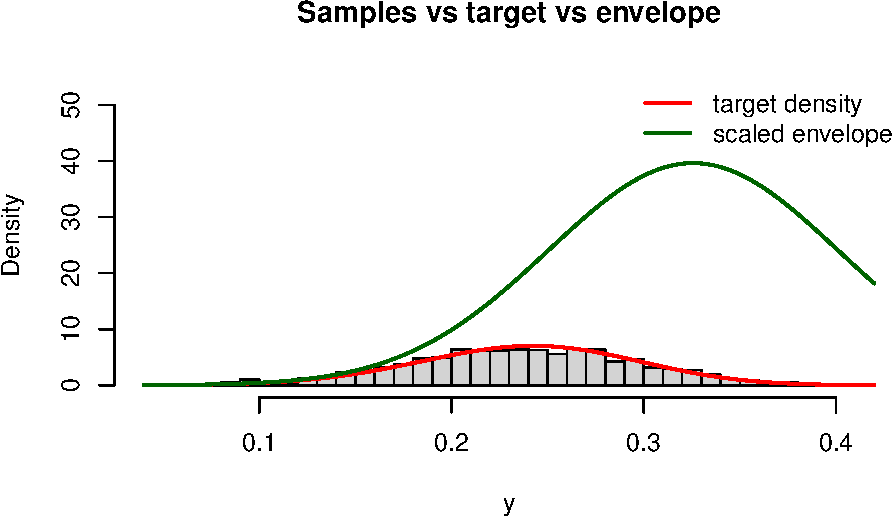
\includegraphics[keepaspectratio]{Presentation-2_files/figure-beamer/unnamed-chunk-1-1.pdf}}
\end{center}

\textbf{Empirical acceptance rate} (fraction accepted out of 200,000 raw
proposals): 0.1341
\end{frame}

\begin{frame}[fragile]{Profiling: Where Does the Time Go?}
\protect\phantomsection\label{profiling-where-does-the-time-go}
Profiling \texttt{log\_rejection\_sample\_vec} (200,000 samples) with
\texttt{Rprof}:

\scriptsize

\begin{Shaded}
\begin{Highlighting}[]
\NormalTok{profvis}\SpecialCharTok{::}\FunctionTok{profvis}\NormalTok{(\{}
  \FunctionTok{log\_rejection\_sample\_vec}\NormalTok{(}
    \AttributeTok{N =} \DecValTok{200000}\NormalTok{,}
    \AttributeTok{rproposal =}\NormalTok{ gaussian\_rproposal,}
    \AttributeTok{log\_accept =}\NormalTok{ log\_accept\_gaussian)}
\NormalTok{\})}
\end{Highlighting}
\end{Shaded}

\normalsize

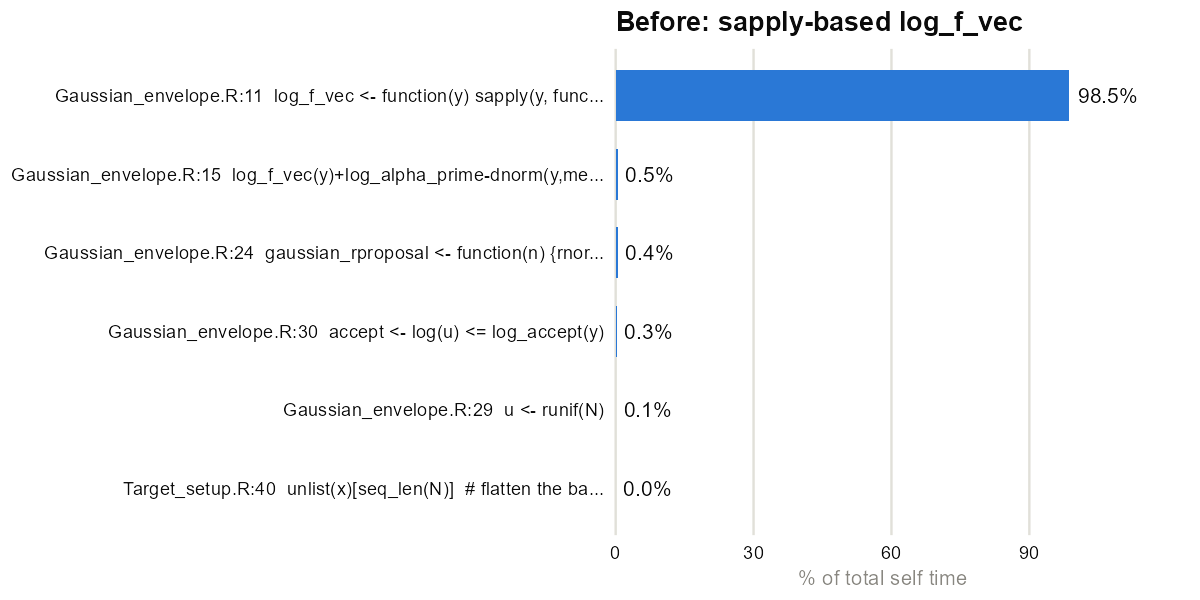
\includegraphics[width=0.9\linewidth,height=\textheight,keepaspectratio]{profiling_before.png}

\textbf{98.5\% of self time is on one line} --- not the math itself, but
calling a fresh R closure once per proposal via \texttt{sapply}.
\end{frame}

\begin{frame}[fragile]{Vectorizing \texttt{log\_f}}
\protect\phantomsection\label{vectorizing-log_f}
\scriptsize

With a 13.4\% acceptance rate, roughly 1.5 million proposals get
evaluated to produce 200,000 accepted samples, each one re-running
\texttt{sapply} and re-fetching \texttt{dat\$z}/\texttt{dat\$x} from
scratch.

\textbf{Idea:} replace the one-proposal-at-a-time \texttt{sapply} with a
single matrix computation covering \emph{all} proposals in a batch at
once.

\begin{Shaded}
\begin{Highlighting}[]
\NormalTok{log\_f\_vec\_faster }\OtherTok{\textless{}{-}} \ControlFlowTok{function}\NormalTok{(y) \{}
\NormalTok{  xy }\OtherTok{\textless{}{-}} \FunctionTok{outer}\NormalTok{(dat}\SpecialCharTok{$}\NormalTok{x, y)         }\CommentTok{\# xy[i,j] = x\_i * y\_j}
  \FunctionTok{colSums}\NormalTok{(dat}\SpecialCharTok{$}\NormalTok{z }\SpecialCharTok{*}\NormalTok{ xy }\SpecialCharTok{{-}} \FunctionTok{exp}\NormalTok{(xy))}
\NormalTok{\}}
\end{Highlighting}
\end{Shaded}

\begin{itemize}
\tightlist
\item
  Exact same output as the original (verified: zero difference)
\item
  \textbf{1.44}\(\times\) faster for the full sampler (19.7s \(\to\)
  13.7s at N = 200\{,\}000)
\end{itemize}

\textbf{Profiling \texttt{log\_f\_vec\_faster}:} the \texttt{sapply}
bottleneck is gone --- runtime is now genuinely inside the vectorized
math itself:

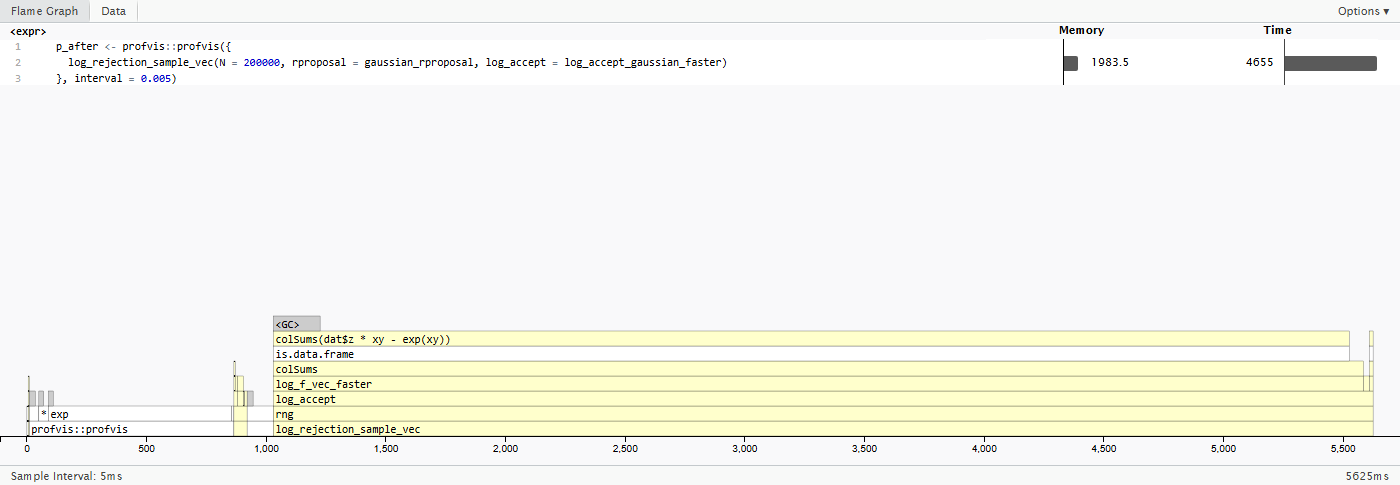
\includegraphics[width=0.9\linewidth,height=\textheight,keepaspectratio]{profiling_after.png}

\normalsize
\end{frame}

\begin{frame}[fragile]{Two C++ Implementations}
\protect\phantomsection\label{two-c-implementations}
\tiny

\begin{columns}[T]
\begin{column}{0.5\linewidth}
\textbf{General} (callback into R for every proposal):

\begin{Shaded}
\begin{Highlighting}[]
\NormalTok{NumericVector rejection\_sample\_cpp}\OperatorTok{(}
    \DataTypeTok{int}\NormalTok{ N}\OperatorTok{,}\NormalTok{ Function rproposal}\OperatorTok{,}\NormalTok{ Function log\_accept}\OperatorTok{)} \OperatorTok{\{}
\NormalTok{  NumericVector out}\OperatorTok{(}\NormalTok{N}\OperatorTok{);}
  \DataTypeTok{double}\NormalTok{ y}\OperatorTok{;}
  \DataTypeTok{bool}\NormalTok{ reject}\OperatorTok{;}

  \ControlFlowTok{for} \OperatorTok{(}\DataTypeTok{int}\NormalTok{ i }\OperatorTok{=} \DecValTok{0}\OperatorTok{;}\NormalTok{ i }\OperatorTok{\textless{}}\NormalTok{ N}\OperatorTok{;} \OperatorTok{++}\NormalTok{i}\OperatorTok{)} \OperatorTok{\{}
    \ControlFlowTok{do} \OperatorTok{\{}
\NormalTok{      y }\OperatorTok{=}\NormalTok{ as}\OperatorTok{\textless{}}\DataTypeTok{double}\OperatorTok{\textgreater{}(}\NormalTok{rproposal}\OperatorTok{(}\DecValTok{1}\OperatorTok{));}
\NormalTok{      reject }\OperatorTok{=}\NormalTok{ log}\OperatorTok{(}\NormalTok{R}\OperatorTok{::}\NormalTok{runif}\OperatorTok{(}\DecValTok{0}\OperatorTok{,} \DecValTok{1}\OperatorTok{))} \OperatorTok{\textgreater{}}
\NormalTok{        as}\OperatorTok{\textless{}}\DataTypeTok{double}\OperatorTok{\textgreater{}(}\NormalTok{log\_accept}\OperatorTok{(}\NormalTok{y}\OperatorTok{));}
    \OperatorTok{\}} \ControlFlowTok{while} \OperatorTok{(}\NormalTok{reject}\OperatorTok{);}
\NormalTok{    out}\OperatorTok{[}\NormalTok{i}\OperatorTok{]} \OperatorTok{=}\NormalTok{ y}\OperatorTok{;}
  \OperatorTok{\}}

  \ControlFlowTok{return}\NormalTok{ out}\OperatorTok{;}
\OperatorTok{\}}
\end{Highlighting}
\end{Shaded}
\end{column}

\begin{column}{0.5\linewidth}
\textbf{Specialized} (target/envelope hardcoded, zero R calls):

\begin{Shaded}
\begin{Highlighting}[]
\NormalTok{NumericVector gaussian\_rejection\_cpp}\OperatorTok{(}
    \DataTypeTok{int}\NormalTok{ N}\OperatorTok{,}\NormalTok{ NumericVector z}\OperatorTok{,}
\NormalTok{    NumericVector x}\OperatorTok{,} \DataTypeTok{double}\NormalTok{ mu}\OperatorTok{,}
    \DataTypeTok{double}\NormalTok{ sigma}\OperatorTok{,} \DataTypeTok{double}\NormalTok{ log\_alpha\_prime}\OperatorTok{)} \OperatorTok{\{}
  \DataTypeTok{int}\NormalTok{ n }\OperatorTok{=}\NormalTok{ z}\OperatorTok{.}\NormalTok{size}\OperatorTok{();}
\NormalTok{  NumericVector out}\OperatorTok{(}\NormalTok{N}\OperatorTok{);}
  \DataTypeTok{double}\NormalTok{ y}\OperatorTok{,}\NormalTok{ log\_fy}\OperatorTok{,}\NormalTok{ log\_gy}\OperatorTok{;}
  \DataTypeTok{bool}\NormalTok{ reject}\OperatorTok{;}

  \ControlFlowTok{for} \OperatorTok{(}\DataTypeTok{int}\NormalTok{ i }\OperatorTok{=} \DecValTok{0}\OperatorTok{;}\NormalTok{ i }\OperatorTok{\textless{}}\NormalTok{ N}\OperatorTok{;} \OperatorTok{++}\NormalTok{i}\OperatorTok{)} \OperatorTok{\{}
    \ControlFlowTok{do} \OperatorTok{\{}
\NormalTok{      y }\OperatorTok{=}\NormalTok{ R}\OperatorTok{::}\NormalTok{rnorm}\OperatorTok{(}\NormalTok{mu}\OperatorTok{,}\NormalTok{ sigma}\OperatorTok{);}
\NormalTok{      log\_fy }\OperatorTok{=} \FloatTok{0.0}\OperatorTok{;}
      \ControlFlowTok{for} \OperatorTok{(}\DataTypeTok{int}\NormalTok{ k }\OperatorTok{=} \DecValTok{0}\OperatorTok{;}\NormalTok{ k }\OperatorTok{\textless{}}\NormalTok{ n}\OperatorTok{;} \OperatorTok{++}\NormalTok{k}\OperatorTok{)}
\NormalTok{        log\_fy }\OperatorTok{+=}\NormalTok{ z}\OperatorTok{[}\NormalTok{k}\OperatorTok{]*}\NormalTok{x}\OperatorTok{[}\NormalTok{k}\OperatorTok{]*}\NormalTok{y }\OperatorTok{{-}}\NormalTok{ exp}\OperatorTok{(}\NormalTok{x}\OperatorTok{[}\NormalTok{k}\OperatorTok{]*}\NormalTok{y}\OperatorTok{);}
\NormalTok{      log\_gy }\OperatorTok{=}\NormalTok{ R}\OperatorTok{::}\NormalTok{dnorm}\OperatorTok{(}\NormalTok{y}\OperatorTok{,}\NormalTok{ mu}\OperatorTok{,}\NormalTok{ sigma}\OperatorTok{,} \KeywordTok{true}\OperatorTok{);}
\NormalTok{      reject }\OperatorTok{=}\NormalTok{ log}\OperatorTok{(}\NormalTok{R}\OperatorTok{::}\NormalTok{runif}\OperatorTok{(}\DecValTok{0}\OperatorTok{,} \DecValTok{1}\OperatorTok{))} \OperatorTok{\textgreater{}}
        \OperatorTok{(}\NormalTok{log\_fy }\OperatorTok{+}\NormalTok{ log\_alpha\_prime }\OperatorTok{{-}}\NormalTok{ log\_gy}\OperatorTok{);}
    \OperatorTok{\}} \ControlFlowTok{while} \OperatorTok{(}\NormalTok{reject}\OperatorTok{);}
\NormalTok{    out}\OperatorTok{[}\NormalTok{i}\OperatorTok{]} \OperatorTok{=}\NormalTok{ y}\OperatorTok{;}
  \OperatorTok{\}}

  \ControlFlowTok{return}\NormalTok{ out}\OperatorTok{;}
\OperatorTok{\}}
\end{Highlighting}
\end{Shaded}
\end{column}
\end{columns}

\normalsize
\end{frame}

\begin{frame}{Benchmarking All Four Versions}
\protect\phantomsection\label{benchmarking-all-four-versions}
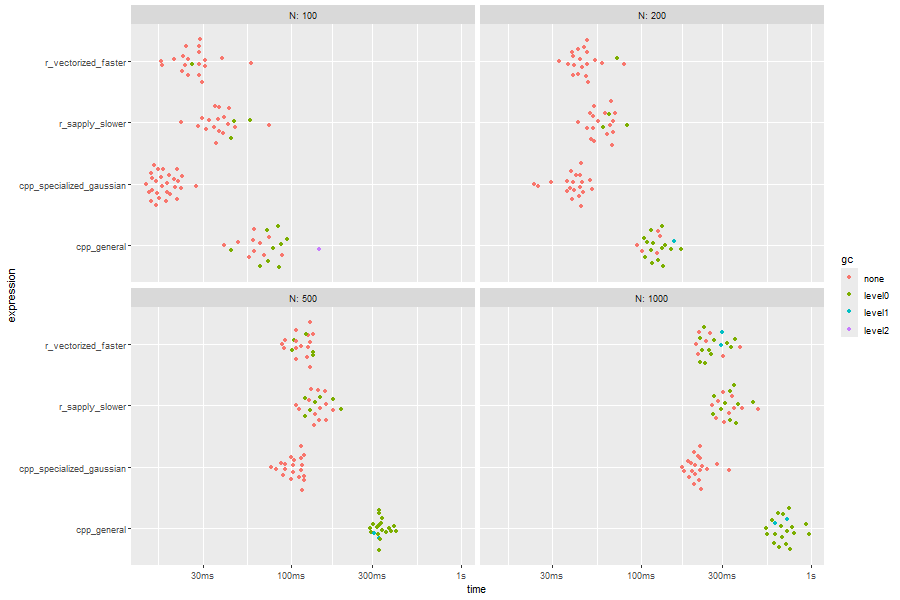
\includegraphics[width=0.85\linewidth,height=\textheight,keepaspectratio]{bench_plot1.png}

The CPP: Generality costs speed, since the general version pays
R-callback overhead on \emph{every} proposal.
\end{frame}

\begin{frame}[fragile]{Benchmarking Across N}
\protect\phantomsection\label{benchmarking-across-n}
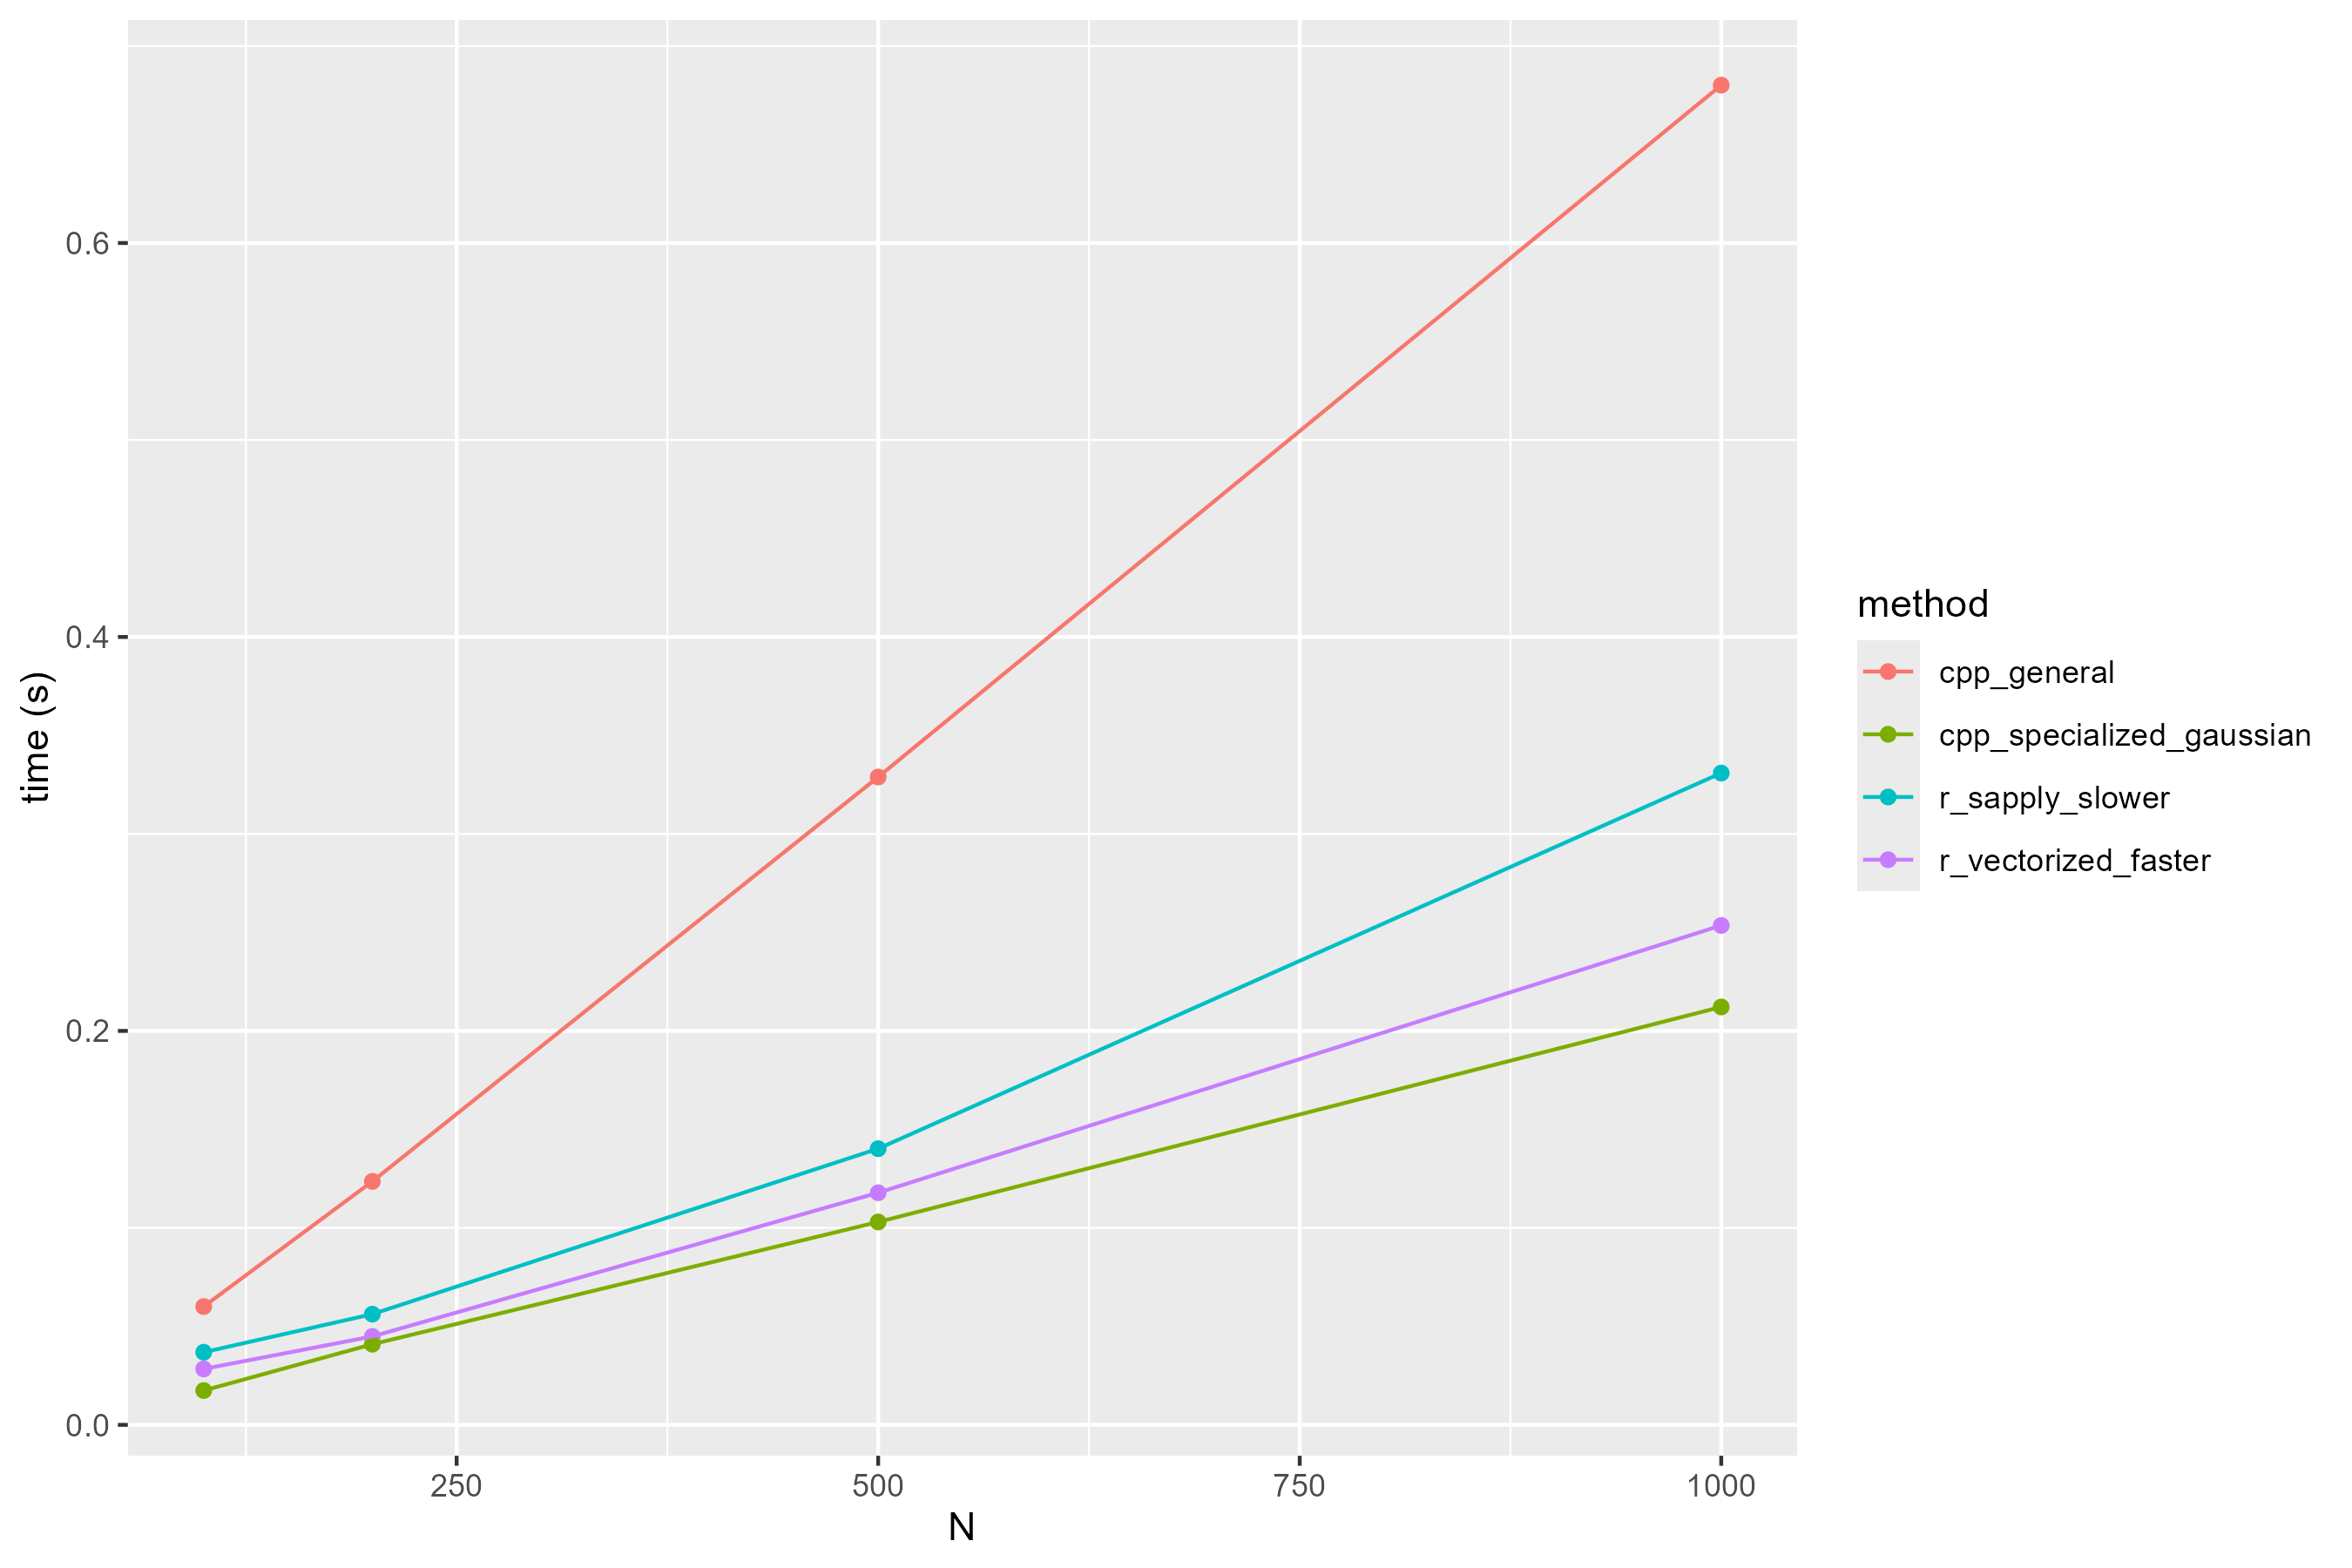
\includegraphics[width=0.75\linewidth,height=\textheight,keepaspectratio]{bench_plot2.png}

\begin{itemize}
\tightlist
\item
  \texttt{cpp\_specialized\_gaussian} and \texttt{r\_vectorized\_faster}
  stay close together
\item
  \texttt{cpp\_general} scales the worst, \texttt{r\_sapply\_slower}
  (original) is a clear second-worst
\end{itemize}
\end{frame}

\begin{frame}{Piecewise Log-Affine Envelope}
\protect\phantomsection\label{piecewise-log-affine-envelope}
Following Section 6.2.1: write \(\ell(y) = \log q(y)\). Then

\[
\ell'(y) = \sum_i x_i(z_i - e^{yx_i}), \qquad \ell''(y) = -\sum_i x_i^2 e^{yx_i} < 0.
\]

So \(\ell\) is \textbf{concave} --- hence we can use it as our proposal
for the piecewise log-affine envelope.

The tangent at \(t_j\) has slope \(a_j = \ell'(t_j)\) and intercept
\(b_j = \ell(t_j) - a_j t_j\).
\end{frame}

\begin{frame}{Building the Envelope}
\protect\phantomsection\label{building-the-envelope}
Adjacent tangents intersect at

\[
c_j = \frac{b_{j+1} - b_j}{a_j - a_{j+1}}.
\]

With \(c_0 = 0\) and \(c_k = \infty\), these define the pieces. The
lowest tangent gives \(V(y) = a_j y + b_j\) on \([c_{j-1}, c_j]\), hence

\[
\alpha'q(y) \leq e^{V(y)}.
\]

Tangency means equality at the chosen points \(\Rightarrow\) we can use
\(\alpha' = 1\) as this works already.
\end{frame}

\begin{frame}{Sampling from the Envelope}
\protect\phantomsection\label{sampling-from-the-envelope}
For a piece with endpoints \(L, R\), its area is

\[
R_j = e^{b_j}\frac{e^{a_j R} - e^{a_j L}}{a_j} \qquad \text{(or } e^{b_j}(R-L) \text{ if } a_j = 0\text{)}.
\]

\begin{itemize}
\tightlist
\item
  These areas give the piecewise-exponential CDF, inverted per-piece to
  sample
\item
  The last slope must be negative for the unbounded right tail to be
  integrable
\end{itemize}
\end{frame}

\begin{frame}{How Many Intervals?}
\protect\phantomsection\label{how-many-intervals}
The book gives no formula --- only a qualitative trade-off:

\begin{quote}
``By increasing the number of \(z\)'s we can make this envelope as tight
as we want. This will lower the rejection probability but also increase
the complexity of simulating from the proposal.''
\end{quote}

Our own measurements confirm this is genuinely an empirical question,
not a closed-form one --- very few points is clearly bad, but beyond a
modest number, more points barely help while adding overhead.
\end{frame}

\begin{frame}[fragile]{Implementing the Log-Affine Envelope (1/2)}
\protect\phantomsection\label{implementing-the-log-affine-envelope-12}
Building the piecewise tangent-line and evaluating it at a point:

\scriptsize

\begin{Shaded}
\begin{Highlighting}[]
\NormalTok{build\_envelope }\OtherTok{\textless{}{-}} \ControlFlowTok{function}\NormalTok{(y\_points) \{}
\NormalTok{  y\_points }\OtherTok{\textless{}{-}} \FunctionTok{sort}\NormalTok{(y\_points)}
\NormalTok{  m }\OtherTok{\textless{}{-}} \FunctionTok{length}\NormalTok{(y\_points)}
\NormalTok{  a }\OtherTok{\textless{}{-}} \FunctionTok{log\_f\_prime\_vec}\NormalTok{(y\_points)}
\NormalTok{  b }\OtherTok{\textless{}{-}} \FunctionTok{log\_f\_vec\_faster}\NormalTok{(y\_points) }\SpecialCharTok{{-}}\NormalTok{ a }\SpecialCharTok{*}\NormalTok{ y\_points}
\NormalTok{  z }\OtherTok{\textless{}{-}}\NormalTok{ (b[}\SpecialCharTok{{-}}\DecValTok{1}\NormalTok{] }\SpecialCharTok{{-}}\NormalTok{ b[}\SpecialCharTok{{-}}\NormalTok{m]) }\SpecialCharTok{/}\NormalTok{ (a[}\SpecialCharTok{{-}}\NormalTok{m] }\SpecialCharTok{{-}}\NormalTok{ a[}\SpecialCharTok{{-}}\DecValTok{1}\NormalTok{])       }\CommentTok{\# tangent intersections c\_j}
  \FunctionTok{list}\NormalTok{(}\AttributeTok{a =}\NormalTok{ a, }\AttributeTok{b =}\NormalTok{ b, }\AttributeTok{z =} \FunctionTok{c}\NormalTok{(}\DecValTok{0}\NormalTok{, z, }\ConstantTok{Inf}\NormalTok{))}
\NormalTok{\}}

\NormalTok{eval\_V }\OtherTok{\textless{}{-}} \ControlFlowTok{function}\NormalTok{(envelope, y) \{}
\NormalTok{  i }\OtherTok{\textless{}{-}} \FunctionTok{findInterval}\NormalTok{(y, envelope}\SpecialCharTok{$}\NormalTok{z)}
\NormalTok{  envelope}\SpecialCharTok{$}\NormalTok{a[i] }\SpecialCharTok{*}\NormalTok{ y }\SpecialCharTok{+}\NormalTok{ envelope}\SpecialCharTok{$}\NormalTok{b[i]}
\NormalTok{\}}
\end{Highlighting}
\end{Shaded}

\normalsize

Since tangency gives equality at each \(t_j\), \(\alpha' = 1\) --- no
separate normalizing-constant step is needed.
\end{frame}

\begin{frame}[fragile]{Implementing the Log-Affine Envelope (2/2)}
\protect\phantomsection\label{implementing-the-log-affine-envelope-22}
Sampling from the piecewise-exponential envelope, then the accept/reject
step:

\tiny

\begin{Shaded}
\begin{Highlighting}[]
\NormalTok{sample\_from\_envelope\_vec }\OtherTok{\textless{}{-}} \ControlFlowTok{function}\NormalTok{(envelope, n) \{}
\NormalTok{  a }\OtherTok{\textless{}{-}}\NormalTok{ envelope}\SpecialCharTok{$}\NormalTok{a; b }\OtherTok{\textless{}{-}}\NormalTok{ envelope}\SpecialCharTok{$}\NormalTok{b; z }\OtherTok{\textless{}{-}}\NormalTok{ envelope}\SpecialCharTok{$}\NormalTok{z}
\NormalTok{  m }\OtherTok{\textless{}{-}} \FunctionTok{length}\NormalTok{(a)}
\NormalTok{  R }\OtherTok{\textless{}{-}} \FunctionTok{numeric}\NormalTok{(m)                              }\CommentTok{\# per{-}piece area under exp(V)}
  \ControlFlowTok{for}\NormalTok{ (i }\ControlFlowTok{in} \FunctionTok{seq\_len}\NormalTok{(m)) \{}
\NormalTok{    lo }\OtherTok{\textless{}{-}}\NormalTok{ z[i]; hi }\OtherTok{\textless{}{-}}\NormalTok{ z[i }\SpecialCharTok{+} \DecValTok{1}\NormalTok{]}
\NormalTok{    R[i] }\OtherTok{\textless{}{-}} \ControlFlowTok{if}\NormalTok{ (}\FunctionTok{is.infinite}\NormalTok{(hi)) }\SpecialCharTok{{-}}\FunctionTok{exp}\NormalTok{(a[i]}\SpecialCharTok{*}\NormalTok{lo }\SpecialCharTok{+}\NormalTok{ b[i]) }\SpecialCharTok{/}\NormalTok{ a[i]}
            \ControlFlowTok{else}\NormalTok{ (}\FunctionTok{exp}\NormalTok{(a[i]}\SpecialCharTok{*}\NormalTok{hi }\SpecialCharTok{+}\NormalTok{ b[i]) }\SpecialCharTok{{-}} \FunctionTok{exp}\NormalTok{(a[i]}\SpecialCharTok{*}\NormalTok{lo }\SpecialCharTok{+}\NormalTok{ b[i])) }\SpecialCharTok{/}\NormalTok{ a[i]}
\NormalTok{  \}}
\NormalTok{  Q }\OtherTok{\textless{}{-}} \FunctionTok{cumsum}\NormalTok{(R); d }\OtherTok{\textless{}{-}}\NormalTok{ Q[m]}
\NormalTok{  target\_area }\OtherTok{\textless{}{-}} \FunctionTok{runif}\NormalTok{(n) }\SpecialCharTok{*}\NormalTok{ d}
\NormalTok{  i }\OtherTok{\textless{}{-}} \FunctionTok{pmin}\NormalTok{(}\FunctionTok{findInterval}\NormalTok{(target\_area, Q) }\SpecialCharTok{+} \DecValTok{1}\NormalTok{, m)}
\NormalTok{  Q\_full }\OtherTok{\textless{}{-}} \FunctionTok{c}\NormalTok{(}\DecValTok{0}\NormalTok{, Q)}
\NormalTok{  area\_into\_piece }\OtherTok{\textless{}{-}}\NormalTok{ target\_area }\SpecialCharTok{{-}}\NormalTok{ Q\_full[i]}
\NormalTok{  rhs }\OtherTok{\textless{}{-}}\NormalTok{ area\_into\_piece }\SpecialCharTok{*}\NormalTok{ a[i] }\SpecialCharTok{+} \FunctionTok{exp}\NormalTok{(a[i] }\SpecialCharTok{*}\NormalTok{ z[i] }\SpecialCharTok{+}\NormalTok{ b[i])}
\NormalTok{  (}\FunctionTok{log}\NormalTok{(rhs) }\SpecialCharTok{{-}}\NormalTok{ b[i]) }\SpecialCharTok{/}\NormalTok{ a[i]                     }\CommentTok{\# invert piecewise{-}exp CDF}
\NormalTok{\}}

\NormalTok{sample\_fixed\_random }\OtherTok{\textless{}{-}} \ControlFlowTok{function}\NormalTok{(N, envelope) \{}
\NormalTok{  y }\OtherTok{\textless{}{-}} \FunctionTok{sample\_from\_envelope\_vec}\NormalTok{(envelope, N)}
\NormalTok{  accept }\OtherTok{\textless{}{-}} \FunctionTok{log}\NormalTok{(}\FunctionTok{runif}\NormalTok{(N)) }\SpecialCharTok{\textless{}=} \FunctionTok{log\_f\_vec\_faster}\NormalTok{(y) }\SpecialCharTok{{-}} \FunctionTok{eval\_V}\NormalTok{(envelope, y)}
\NormalTok{  y[accept]}
\NormalTok{\}}
\NormalTok{sample\_fixed\_vec }\OtherTok{\textless{}{-}} \FunctionTok{rng\_vec}\NormalTok{(sample\_fixed\_random)}
\end{Highlighting}
\end{Shaded}

\normalsize
\end{frame}

\begin{frame}[fragile]{Finding the Best Number of Intervals}
\protect\phantomsection\label{finding-the-best-number-of-intervals}
A fixed, non-adaptive grid of \(m\) tangent points, spaced over
\([0, \hat{y} + 3\hat{\sigma}]\) (mode \(\pm\) curvature-based spread).
More points yields a higher acceptance rate, but each proposal also
costs more to build and sample from.

\scriptsize

\begin{Shaded}
\begin{Highlighting}[]
\NormalTok{time\_for\_m }\OtherTok{\textless{}{-}} \ControlFlowTok{function}\NormalTok{(m, N, }\AttributeTok{min\_iterations =} \DecValTok{5}\NormalTok{) \{}
\NormalTok{  y\_points }\OtherTok{\textless{}{-}} \FunctionTok{seq}\NormalTok{(}\FloatTok{0.02}\NormalTok{, y\_hat }\SpecialCharTok{+} \DecValTok{3} \SpecialCharTok{*}\NormalTok{ sd\_hat, }\AttributeTok{length.out =}\NormalTok{ m)}
\NormalTok{  envelope }\OtherTok{\textless{}{-}} \FunctionTok{build\_envelope}\NormalTok{(y\_points)}
\NormalTok{  b }\OtherTok{\textless{}{-}}\NormalTok{ bench}\SpecialCharTok{::}\FunctionTok{mark}\NormalTok{(}
    \FunctionTok{sample\_fixed\_vec}\NormalTok{(N, }\AttributeTok{envelope =}\NormalTok{ envelope),}
    \AttributeTok{min\_iterations =}\NormalTok{ min\_iterations, }\AttributeTok{check =} \ConstantTok{FALSE}
\NormalTok{  )}
  \FunctionTok{data.frame}\NormalTok{(}\AttributeTok{m =}\NormalTok{ m, }\AttributeTok{time =} \FunctionTok{as.numeric}\NormalTok{(b}\SpecialCharTok{$}\NormalTok{median), }\AttributeTok{acceptance\_rate =}\NormalTok{ ...)}
\NormalTok{\}}

\NormalTok{find\_best\_m }\OtherTok{\textless{}{-}} \ControlFlowTok{function}\NormalTok{(candidate\_ms, N, }\AttributeTok{min\_iterations =} \DecValTok{5}\NormalTok{, }\AttributeTok{acc\_threshold =} \FloatTok{0.99}\NormalTok{) \{}
\NormalTok{  results }\OtherTok{\textless{}{-}} \FunctionTok{do.call}\NormalTok{(rbind, }\FunctionTok{lapply}\NormalTok{(candidate\_ms, time\_for\_m, }\AttributeTok{N =}\NormalTok{ N,}
                                    \AttributeTok{min\_iterations =}\NormalTok{ min\_iterations))}
\NormalTok{  above }\OtherTok{\textless{}{-}}\NormalTok{ results[results}\SpecialCharTok{$}\NormalTok{acceptance\_rate }\SpecialCharTok{\textgreater{}=}\NormalTok{ acc\_threshold, ]}
  \FunctionTok{list}\NormalTok{(}\AttributeTok{results =}\NormalTok{ results, }\AttributeTok{best =}\NormalTok{ above[}\FunctionTok{which.min}\NormalTok{(above}\SpecialCharTok{$}\NormalTok{m), ])}
\NormalTok{\}}

\NormalTok{out }\OtherTok{\textless{}{-}} \FunctionTok{find\_best\_m}\NormalTok{(}\FunctionTok{c}\NormalTok{(}\DecValTok{2}\NormalTok{, }\DecValTok{3}\NormalTok{, }\DecValTok{5}\NormalTok{, }\DecValTok{8}\NormalTok{, }\DecValTok{12}\NormalTok{, }\DecValTok{20}\NormalTok{, }\DecValTok{30}\NormalTok{, }\DecValTok{50}\NormalTok{, }\DecValTok{60}\NormalTok{, }\DecValTok{70}\NormalTok{), }\AttributeTok{N =} \DecValTok{1000}\NormalTok{, }\AttributeTok{min\_iterations =} \DecValTok{30}\NormalTok{)}
\end{Highlighting}
\end{Shaded}

\normalsize
\end{frame}

\begin{frame}{How the Best m Was Chosen}
\protect\phantomsection\label{how-the-best-m-was-chosen}
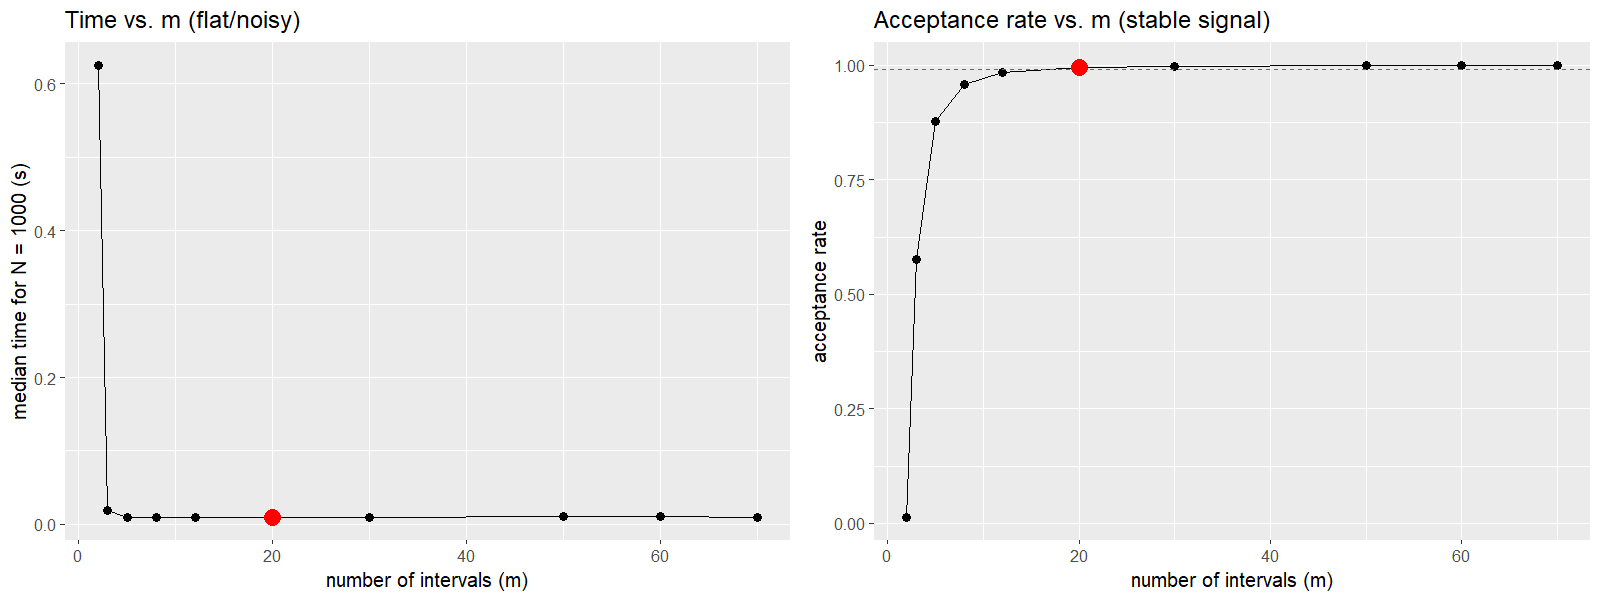
\includegraphics[width=1\linewidth,height=\textheight,keepaspectratio]{sweep_plot.png}

Time (left) drops sharply from \(m=2\) to \(m=5\), and is then mostly
flat --- re-running the sweep does not reliably pick the same argmin.
Acceptance rate (right) is monotone and stable, so we take the smallest
\(m\) crossing 99\% (dashed line): \(m =\) 20 (red point).
\end{frame}

\begin{frame}{Correctness Check: Log-Affine Envelope}
\protect\phantomsection\label{correctness-check-log-affine-envelope}
\begin{center}
\pandocbounded{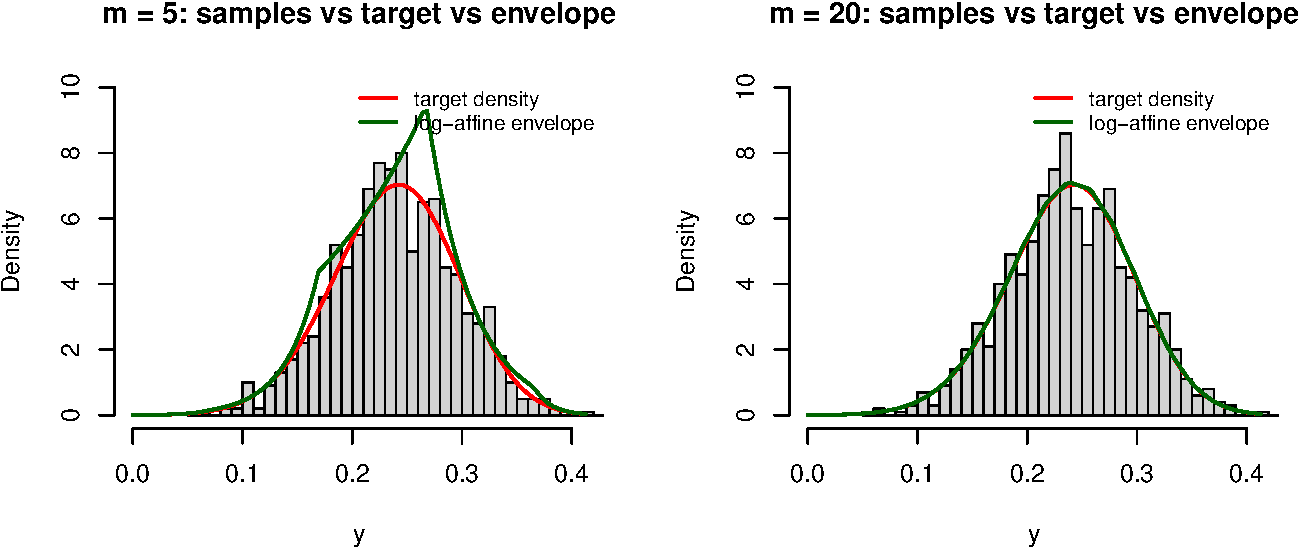
\includegraphics[keepaspectratio]{Presentation-2_files/figure-beamer/unnamed-chunk-3-1.pdf}}
\end{center}

With \(m = 5\) the envelope is visibly loose (lower acceptance rate); at
the best \(m\) it hugs the target density much more tightly.
\end{frame}

\begin{frame}{Benchmarking: Log-Affine vs.~Gaussian}
\protect\phantomsection\label{benchmarking-log-affine-vs.-gaussian}
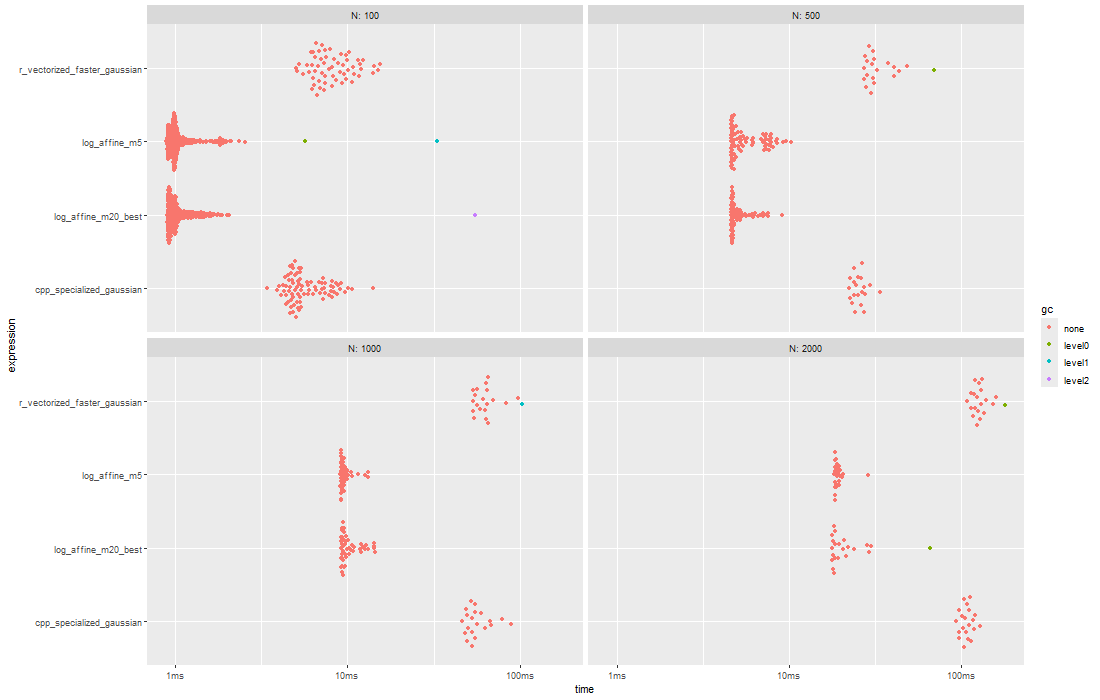
\includegraphics[width=0.7\linewidth,height=\textheight,keepaspectratio]{bench_plot3.png}

Comparing all four methods at N = 100, 500, 1000, 2000 (min. 20
iterations each) --- both log-affine variants are consistently faster
than either Gaussian implementation, and the gap widens as N grows.
\end{frame}

\begin{frame}[fragile]{Benchmarking Across N}
\protect\phantomsection\label{benchmarking-across-n-1}
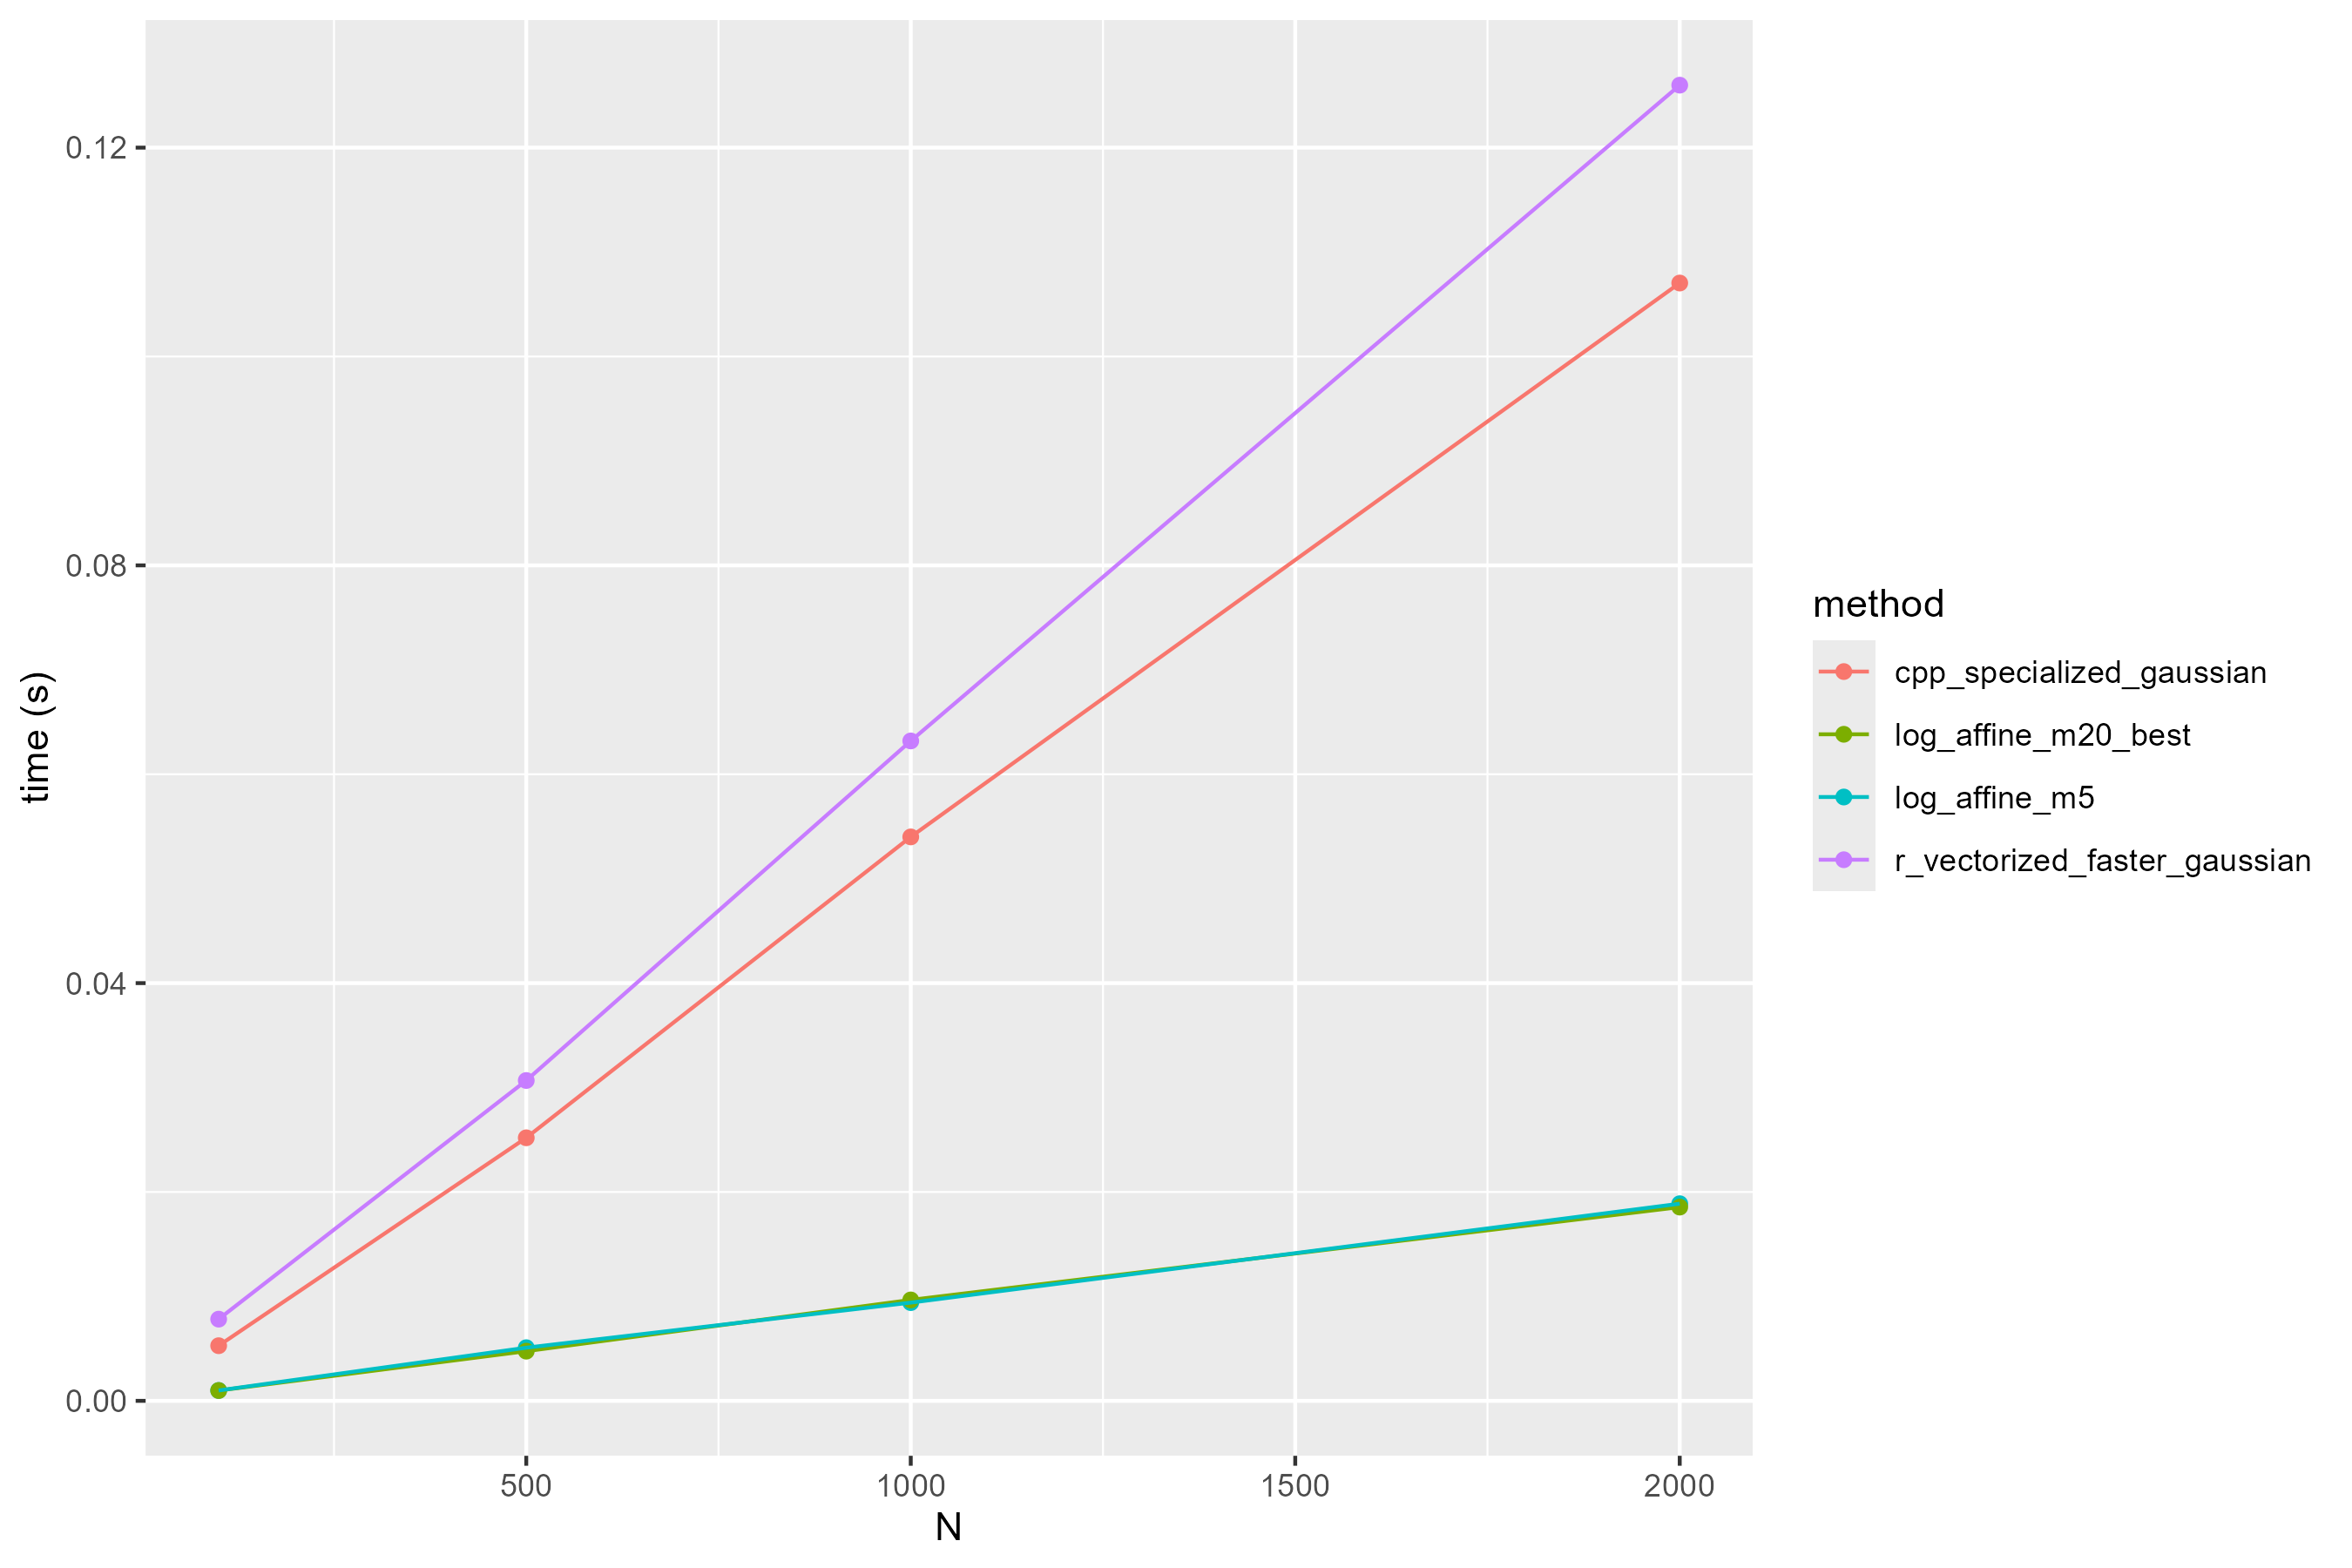
\includegraphics[width=0.6\linewidth,height=\textheight,keepaspectratio]{bench_plot4.png}

Both log-affine variants beat \texttt{cpp\_specialized\_gaussian} and
\texttt{r\_vectorized\_faster\_gaussian} at every N, and the gap widens
as N grows.
\end{frame}

\begin{frame}{Benchmarking Across N: Why}
\protect\phantomsection\label{benchmarking-across-n-why}
\textbf{Acceptance rate decides the speed --- not the language.}

{\def\LTcaptype{none} % do not increment counter
\begin{longtable}[]{@{}ll@{}}
\toprule\noalign{}
Method & Acceptance \\
\midrule\noalign{}
\endhead
Gaussian envelope (R or C++) & \(\approx\) 13\% \\
Log-affine, \(m=5\) & 87.7\% \\
Log-affine, best \(m\) & 99.5\% \\
\bottomrule\noalign{}
\end{longtable}
}
\end{frame}

\begin{frame}{Questions \& Further Work}
\protect\phantomsection\label{questions-further-work}
\textbf{Questions?}

\textbf{Further work:}

\begin{itemize}
\tightlist
\item
  The log-affine sampler is still written in R, while the Gaussian
  envelope also has a C++ version. Rewriting the log-affine sampler in
  C++ could make it even faster
\item
  We placed the tangent points evenly spaced across the range. This may
  not be the best choice --- spacing them based on where the curve is
  more curved could give a tighter envelope with fewer points
\end{itemize}
\end{frame}




\end{document}
